
%使用XeLaTeX编译
%版权所有,翻版必究
%本文件由程序自动生成,任何修改将被覆盖
%2019 年 01 月 23 日




\FloatBarrier
\section{
曲线图导引
}\label{c000017s01}


曲线图(Qt Charts)模块默认并不被安装,
但是它非常有用,
读者应当总是安装这个模块。

要使用Qt Charts模块需要在QML头添加:\begin{littlelongworld}
import QtCharts 2.3
\end{littlelongworld}
并在工程文件添加:\begin{littlelongworld}
QT {\sourcefonttwo{}+}{\sourcefonttwo{}=} charts
\end{littlelongworld}
\hspace*{\parindent}\filesourcenumbernameone\ \ref{f000080}展示
了一个简单的Qt Charts模块的应用。

%../chapter08/firstchart/the_book.png
%begin图片
\begin{figure}[htb] %浮动体 here and top ...
%there must use marginnote ...
\marginnote{\setlength\fboxsep{2pt}\fbox{\footnotesize{\kaishu\figurename\,}\footnotesize{\ref{p000049}}}}\centering %中心对齐
\setlength\fboxsep{0pt}\fcolorbox[rgb]{0,0,0}{0.97,0.98,0.99}{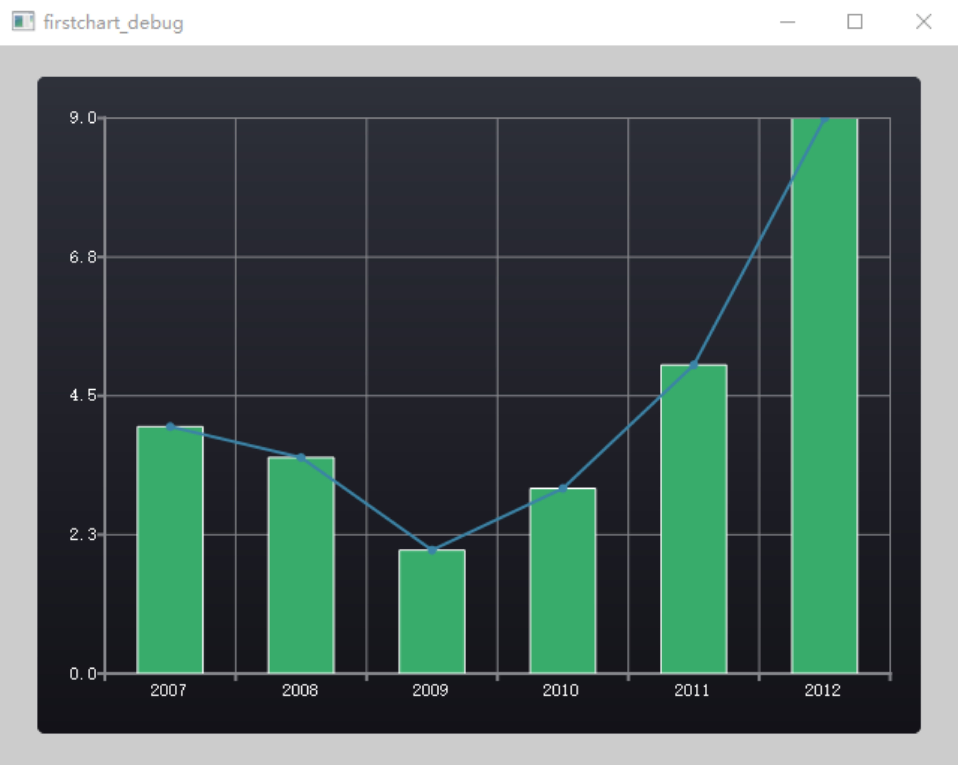
\includegraphics[width=0.95\textwidth]{the_book_image/p000049.pdf}} %图片路径
\caption{QtCharts} %标题
\label{p000049} %索引
\end{figure}
%end图片


%../chapter08/firstchart/myqml/firstchart/main.qml
%\begin{spacing}{1.0}
\refstepcounter{filesourcenumber}\label{f000080}    %增加源代码编号
\FloatBarrier                                  %强制完成浮动体布局
\begin{thebookfilesourceone}[escapeinside={(*@}{@*)},
caption=GoodLuck,
title=\filesourcenumbernameone \thefilesourcenumber
]
/*firstchart/main.qml*/
import QtQuick 2.9
import QtCharts 2.3

Rectangle {

    id : idRoot
    width: 640;
    height: 480;
    color: Qt.rgba(0.8,0.8,0.8,1);

    ChartView{
        anchors.centerIn: parent ;
        width: parent.width * 0.95 ;
        height: parent.height * 0.95 ;
        theme: ChartView.ChartThemeDark
        antialiasing: true
        dropShadowEnabled : true
        legend.visible : false
        animationOptions :ChartView.AllAnimations

        BarSeries {
            id: idBar
            axisX: BarCategoryAxis {
                categories: [
                    "2007",
                    "2008",
                    "2009",
                    "2010",
                    "2011",
                    "2012" ] }
            BarSet {
                label: qsTr( "FirstChart" );
                values: [4, 3.5, 2, 3, 5, 9]
            }
        }

        LineSeries{
            XYPoint { x: 0; y: 4 }
            XYPoint { x: 1; y: 3.5 }
            XYPoint { x: 2; y: 2 }
            XYPoint { x: 3; y: 3 }
            XYPoint { x: 4; y: 5 }
            XYPoint { x: 5; y: 9 }
            axisX: idBar.axisX
            axisY: idBar.axisY
            pointsVisible: true
            pointLabelsVisible : false
        }

    }

}/*~Rectangle*/(*@\marginpar[\hfill\setlength\fboxsep{2pt}\fbox{\footnotesize{\kaishu\parbox{1em}{\setlength{\baselineskip}{2pt}\filesourcenumbernameone}}\footnotesize{\thefilesourcenumber}}]{\setlength\fboxsep{2pt}\fbox{\footnotesize{\kaishu\parbox{1em}{\setlength{\baselineskip}{2pt}\filesourcenumbernameone}}\footnotesize{\thefilesourcenumber}}}@*)\end{thebookfilesourceone}          %抄录环境
\addtocounter{lstlisting}{-1}   %sub lstlisting counter ...
%\end{spacing}


\begin{comment}
介绍代码..........................
\end{comment}

如\filesourcenumbernameone\ \ref{f000080}所
示:
\begin{itemize}
\item 第12行使用ChartView作为
Qt Charts各类曲线的
视图。
    \begin{itemize}
\item 第16行定义了ChartView的主题。
\item 第19行要求隐藏
图例。
\item 第20行启用所有动画。
    \end{itemize}
\item 第22行、第38行
分别定义了柱状图和折线图。
\item 第45\raisebox{0.16ex}{\sourcefonttwo\~{}}46行
规定折线图使用柱状图的坐标系。

\end{itemize}

视图、
曲线、
坐标轴、
图例、
动画
与
主题。
这些是Qt Charts支持良好的部分。

除此之外,Qt Charts也支持
输入设备(比如鼠标键盘)响应和
移动视图。

有时候需要给Qt Charts增加一些额外自定义元素,
那么就不得不深入Qt Charts源码并多费心思。
毕竟Qt Charts是为QGraphicsView而设计的,
对于Qt Quick而言,Qt Charts的
一些设计就过于呆板。


\begin{comment}
!!!!Qt Charts Overview 

AbstractAxis 
A base type used for specialized axis types
AbstractBarSeries 
An abstract parent type for all bar series types
AbstractSeries 
Base type for all Qt Chart series types
AreaSeries 
Presents data in area charts
BarCategoryAxis 
Adds categories to a chart's axes
BarSeries 
Presents a series of data as vertical bars grouped by category
BarSet
Represents one set of bars in a bar chart
BoxPlotSeries
Presents data in box-and-whiskers charts
BoxSet
Represents one item in a box-and-whiskers chart
CandlestickSeries
Represents a series of data as candlesticks
CandlestickSet
Represents a single candlestick item in a candlestick chart
CategoryAxis
Places named ranges on the axis
CategoryRange
Defines a range on a category axis
ChartView
Manages the graphical representation of the chart's series, legends, and axes
DateTimeAxis
Adds dates and times to a chart's axis
HBarModelMapper
Horizontal model mapper for bar series
HBoxPlotModelMapper
Horizontal model mapper for box plot series
HCandlestickModelMapper
Horizontal model mapper for a candlestick series
HPieModelMapper
Horizontal model mapper for pie series
HXYModelMapper
A horizontal model mapper for XYSeries
HorizontalBarSeries
Presents a series of data as horizontal bars grouped by category
HorizontalPercentBarSeries
Presents a series of categorized data as a percentage of each category
HorizontalStackedBarSeries
Presents a series of data as stacked horizontal bars, with one bar per category
Legend
Displays the legend of a chart
LineSeries
Presents data in line charts
LogValueAxis
Adds a logarithmic scale to a chart's axis
Margins
Defines margins between the edge of the chart rectangle and the plot area
PercentBarSeries
Presents a series of categorized data as a percentage of each category
PieSeries
Presents data in pie charts
PieSlice
Represents a single slice in a pie series
PolarChartView
Presents data in polar charts
ScatterSeries
Type presents data in scatter charts
SplineSeries
Presents data as spline charts
StackedBarSeries
Presents a series of data as vertically stacked bars, with one bar per category
VBarModelMapper
Vertical model mapper for bar series
VBoxPlotModelMapper
Vertical model mapper for box plot series
VCandlestickModelMapper
Vertical model mapper for a candlestick series
VPieModelMapper
Vertical model mapper for pie series
VXYModelMapper
A vertical model mapper for XYSeries
ValueAxis
Adds values to a chart's axes
XYPoint
Initializes XY-series coordinate data
XYSeries
A base type for line, spline, and scatter series
\end{comment}    



% ______all_key_words
% the_book_chapter the_book_subsection the_book_subsubsection
% the_book_section the_book_image the_book_table
% the_book_file the_book_tree_file the_book_command_file
% littlelongworld tabbing ref
% figurename tablename filesourcenumbernameone
% treeindexnumbernameone commandnumbernameone footnote
% item itemize comment textbullet
% \hspace*{\parindent}
% FloatBarrier







%使用XeLaTeX编译
%版权所有,翻版必究
%本文件由程序自动生成,任何修改将被覆盖
%2019 年 01 月 23 日



